\documentclass[a4paper,11pt]{article}
\usepackage{amsmath,amssymb}
\usepackage[a4paper,left=19mm,right=19mm,top=40mm,bottom=40mm]{geometry}
\usepackage{txfonts}
\usepackage{kotex}
\usepackage{graphicx}
\usepackage{algorithm}
\usepackage{algpseudocode}
\usepackage{fancyvrb}

\begin{document}
\title{자료구조 HW7}
\author{B935394 컴퓨터공학과 장준희}
\maketitle
\newpage

\section{Binary Tree}
\ \ 이번 과제는 이진트리의 순회(preorder, inorder, postorder,levelorder)를 각각 구현하는 것이였다. 트리를 순회하기 위해서는 트리의 구조가 어떻게 생겼는지부터 이해하는 것이 필수적이라고 생각했기때문에 주어진 insert함수를 이해하는 것부터 시작했다.(검은 글씨와 그림)\\
\begin{figure}[h]
\begin{center}
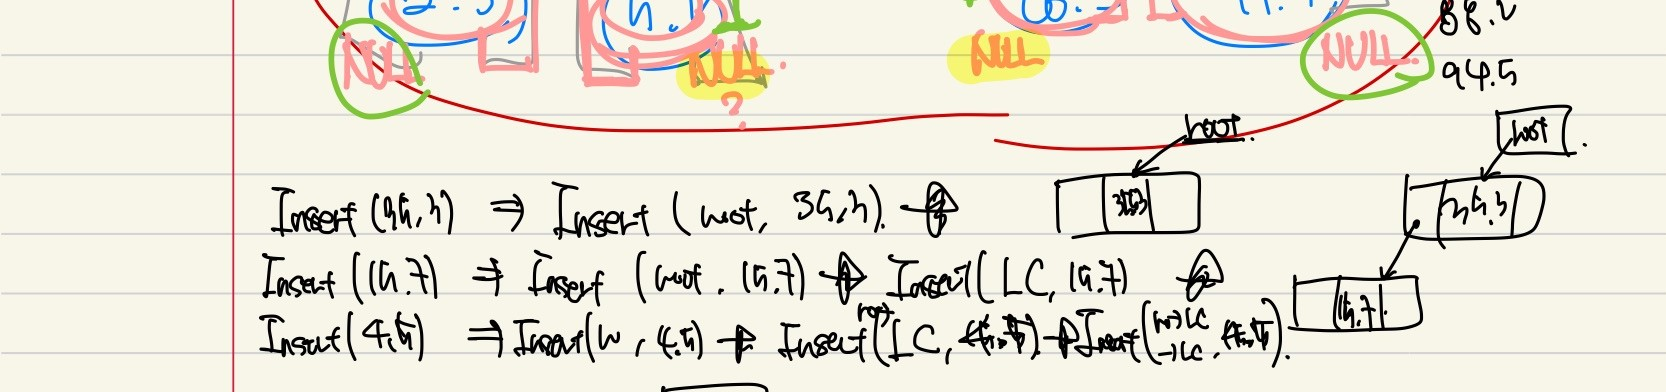
\includegraphics[width=0.7\textwidth]{bt_insert}
\caption{Insert}
\label{fig:fig1}
\end{center}
\end{figure} 
\\\ \ 하나씩 확인해보며, 실행을 확인해보니 그다지 어렵지 않았기에, 빠르게 각 순회들을 구현했다.다만 Inorder함수는 재귀적방법을 쓰면 안됐기때문에, 책에 나와있는 비재귀적 Inorder함수의 구현을 따왔다.
\begin{Verbatim}
------------------------------------------------------
template <class T>
void Tree<T>::Preorder(Node<T> *ptr){
    if(ptr){
        Visit(ptr);		//V
        Preorder(ptr->leftChild);		//L
        Preorder(ptr->rightChild);		//R
    }
}
------------------------------------------------------
template <class T>
void Tree<T>::Inorder(Node<T> *ptr){
    stack<Node<T>*> s;		//노드를 담을 스택
    Node<T> * currentNode = root;	//루트가 가리키는 노드에서 시작			
    while(1){
        while(currentNode){    //가리키는 노드가 있는한 
            s.push(currentNode);		//가리키는 노드를 스택에 푸쉬하고
            currentNode = currentNode->leftChild;  //일단 왼쪽으로 쭉		
        }
        if(s.empty())   return;		//만약 공 스택이라면, 반환
        currentNode = s.top(); s.pop();	//현재 노드에 스택의 맨 위를 주고 팝.
        Visit(currentNode);		//출력
        currentNode = currentNode->rightChild;		//LVR중 R
    }
}
------------------------------------------------------
template <class T>
void Tree<T>::Postorder(Node<T> *ptr){
    if(ptr){
        Postorder(ptr->leftChild);
        Postorder(ptr->rightChild);
        Visit(ptr);
    }
-------------------------------------------------------    
template <class T>
void Tree<T>::Levelorder(){
    queue<Node<T>*> q;
    Node<T> * currentNode=root;
    while(currentNode){
        Visit(currentNode);
        if(currentNode->leftChild){
            q.push(currentNode->leftChild);
        }
        if(currentNode->rightChild){
            q.push(currentNode->rightChild);
        }
        if(q.empty())   return;
        currentNode=q.front(); q.pop(); 
    }
}//위에서부터 읽어가며 읽은 순서대로 출력(FIFO)이므로 큐를 사용한다.
-------------------------------------------------------
\end{Verbatim}
\ \ 그 뒤로 남은 것은 주어진 이진트리를 스레드 이진트리로 바꿔구현한 것이였는데, 책과는 달리 헤더노드를 추가하지는 않고, 스레드 역할만 추가시켰다. 또, 최우측리프노드의 rightchild와 최좌측리프노드의 leftchild에는 어디를 가리키게 하기보다는 0만 담아두었다. 생각한 구조는 다음 그림과 같다. 핑크색이 처음 구현했을 때의 결과이고, 연두색이 수정해야하는 방향이였다. 보라색은 Inorder함수의 구현의 경로였다.\\
 \begin{figure}[h]
\begin{center}
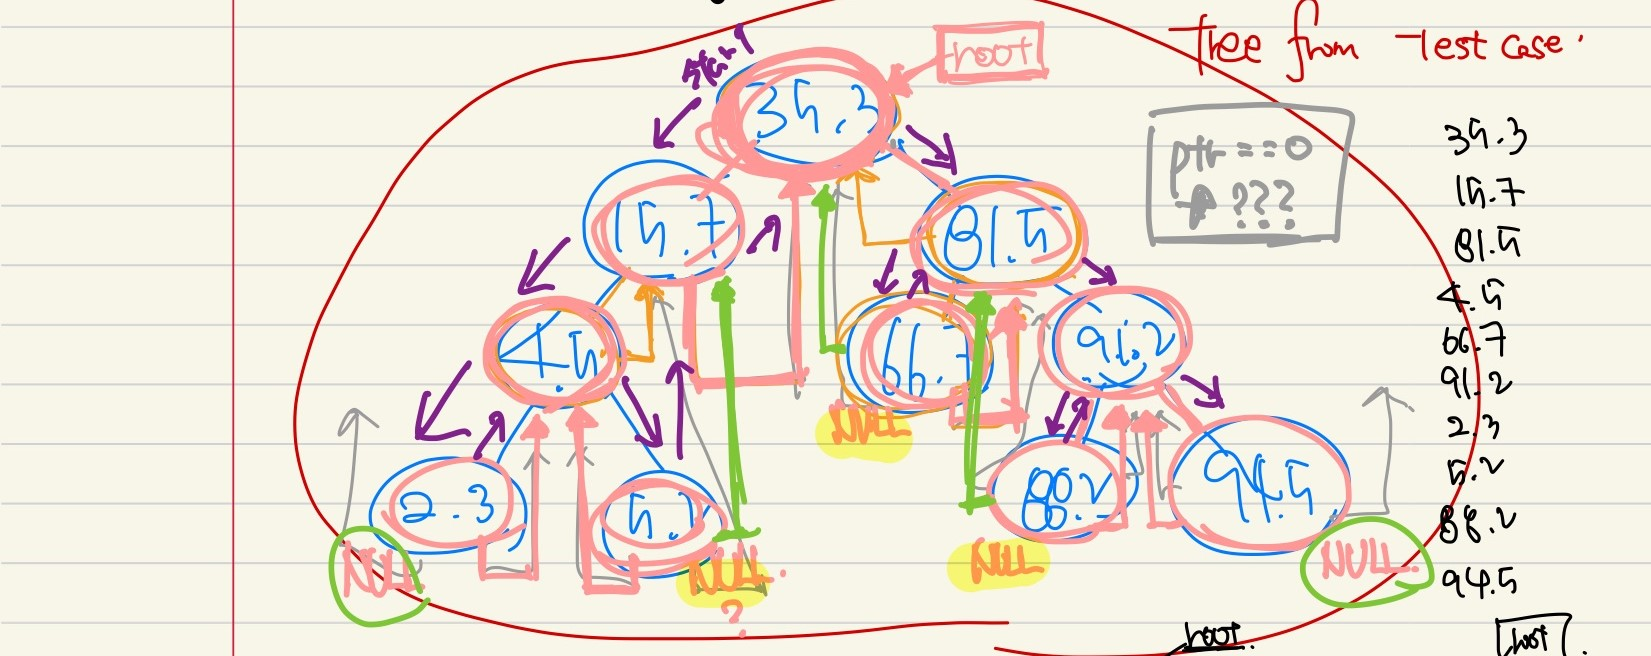
\includegraphics[width=0.7\textwidth]{bt_struct}
\caption{Threaded Binary Tree}
\label{fig:fig2}
\end{center}
\end{figure}
\\\ \ 그림처럼 구현을 하기 위해서는 insert함수의 수정이 필요했다. 과제 pdf의 함수구현처럼 재귀적인 방법을 쓰고 싶었는데, 그렇게 하다보니, 루트노드와 그 자식노드가 처음 생길 때 자식노드의 자식노드 포인터가 루트노드를 가리키다 보니 뺑뺑도는 문제가 발생했다. 또 자식노드가 부모노드를 가리킬 필요가 있었는데 만약에 재귀적인 방법으로 한다면, 그것을 나타낼 길이 필요했다. 그래서 고민을 하던 중 이전 과제에서 static 변수로 이전의 값을 전달하는 것이 생각났다. 따라서 좌/우측에 삽입을 하는 것을 기본으로 루트노드일 때를 추가로 더 생각해주면 되었다.
\begin{Verbatim}
-------------------------------------------------------
void Tree<T>::Insert(Node<T> *&ptr, T &value)
{ //Insert 의 helper 함수
    static Node<T> *temp = 0;
    static bool check = 0;
    static bool visitRoot=false;
    Node<T> *tempChild=0;
    //리프노트일때VS리프노트가 아닐때-->이 조건이 무엇인가??
    if(ptr==root&&visitRoot==false){
        visitRoot=true;
        if(root==0){
            ptr=new Node<T>(value);
            temp=ptr;
        }
        else{
            if (value < ptr->data)
            {
                check = 0;
                temp = ptr;
                Insert(ptr->leftChild, value);
            }
            else if (value > ptr->data)
            {
                check = 1;
                temp = ptr;
                Insert(ptr->rightChild, value);
            }
            else
                cout << "Duplicate value " << value << " ignored\n" << endl;
        }
    }//루트
    else if(check==0){
        if(temp->leftThreaded==true){
            tempChild=temp->leftChild;
            ptr=new Node<T>(value);
            ptr->rightChild=temp;
            ptr->leftChild=tempChild;
            temp->leftThreaded=false;
        }
        else{
            if (value < ptr->data)
            {
                check = 0;
                temp = ptr;
                Insert(ptr->leftChild, value);
            }
            else if (value > ptr->data)
            {
                check = 1;
                temp = ptr;
                Insert(ptr->rightChild, value);
            }
            else
                cout << "Duplicate value " << value << " ignored\n" << endl;

        }
    }//좌측
    else if(check==1){
        if(temp->rightThreaded==true){
            tempChild=temp->rightChild;
            ptr=new Node<T> (value);
            ptr->leftChild=temp;
            ptr->rightChild=tempChild;
            temp->rightThreaded=false;
        }
        else{
            if (value < ptr->data)
            {
                check = 0;
                temp = ptr;
                Insert(ptr->leftChild, value);
            }
            else if (value > ptr->data)
            {
                check = 1;
                temp = ptr;
                Insert(ptr->rightChild, value);
            }
            else
                cout << "Duplicate value " << value << " ignored\n" << endl;
        }
    }//우측
    visitRoot=false;
}
-------------------------------------------------------
\end{Verbatim}
\ \ 다만 노드에서 child노드가 단순히 자식노드를 가리키지만은 않게됐으므로, 각 순회방법에 있어서도 조금씩은 수정이 필요했고, 다른 세 함수같은 경우는 자식을 가리키는지 혹은 인오더후속자를 가리키는지만 추가해주면 됐지만, inorder같은 경우는 이전 방법과는 아예다르게 경로를 주욱 따라가게 해야했다.
\begin{Verbatim}
-------------------------------------------------------
template <class T>
void Tree<T>::Preorder(Node<T> *ptr){
    if(ptr){
        Visit(ptr);
        if(ptr->leftThreaded==false)
            Preorder(ptr->leftChild);
        if(ptr->rightThreaded==false)
            Preorder(ptr->rightChild);
    }
}
-------------------------------------------------------
template <class T>
void Tree<T>::Inorder(Node<T> *ptr){
    Node<T> *currentNode=root;
    static bool visitRoot=false;
    while(currentNode->rightChild!=0){
        Node<T> * temp;
        if(visitRoot==false){
            temp=currentNode;
            visitRoot=true;
        }
        else
            temp=currentNode->rightChild;       
        if(!currentNode->rightThreaded)
            while(!temp->leftThreaded)temp=temp->leftChild;
        currentNode=temp;
        Visit(currentNode);
    }    
}
-------------------------------------------------------
template <class T>
void Tree<T>::Postorder(Node<T> *ptr){
    if(ptr){
        if(ptr->leftThreaded==false)
            Postorder(ptr->leftChild);
        if(ptr->rightThreaded==false)
            Postorder(ptr->rightChild);
        Visit(ptr);
    }
}
-------------------------------------------------------
template <class T>
void Tree<T>::Levelorder(){
    queue<Node<T>*> q;
    Node<T> * currentNode=root;
    while(currentNode){
        Visit(currentNode);
        if(currentNode->leftChild&&currentNode->leftThreaded==false){
            q.push(currentNode->leftChild);
        }
        if(currentNode->rightChild&&currentNode->rightThreaded==false){
            q.push(currentNode->rightChild);
        }
        if(q.empty())   return;
        currentNode=q.front(); q.pop(); 
    }
}
-------------------------------------------------------
\end{Verbatim}
\section{과제하면서 어려웠던 점}
\begin{itemize}
\item 포인터, 참조자, 템플릿, 구조체, 클래스 등을 더 잘 이해하고 공부할 필요가 있다고 생각했다.
\item 위에서는 간략하게 설명했지만 insert함수를 구현할 때, 어떻게 분류할지, 어떤 조건식을 써야 좋을지 등을 한참을 고민했었다. 이런 것을 쉽게 해내고 싶다.
\end{itemize}
\end{document}